% !TeX root = OptCuts.tex

\section{Results and Discussion}
\label{sec:results}

\minchen{Text possibly needed in the description of how we handle global bijectivity:
When computing $\hat{f}_e$, besides also including the one-ring triangles on the scaffold mesh for computing energy decrease, we also need to move the splitted vertices slightly apart to leave room for inserting new scaffold mesh triangles.}
\minchen{Add energy plot to show convergence?}


\subsection{Method Evaluation}

We evaluate our method with/without global bijectivity by running them on 70 input surfaces including both disk-topology and closed surfaces (some are with \minchen{[TODO] high genus}), setting $b_d$ to $4.2$, $4.1$, and $4.05$ (Figure~\ref{fig:our_impressive_results}). Our methods automatically generate high quality UV maps given any distortion bounds for all inputs without any user assistance.

\begin{figure*}[!h]
\centering
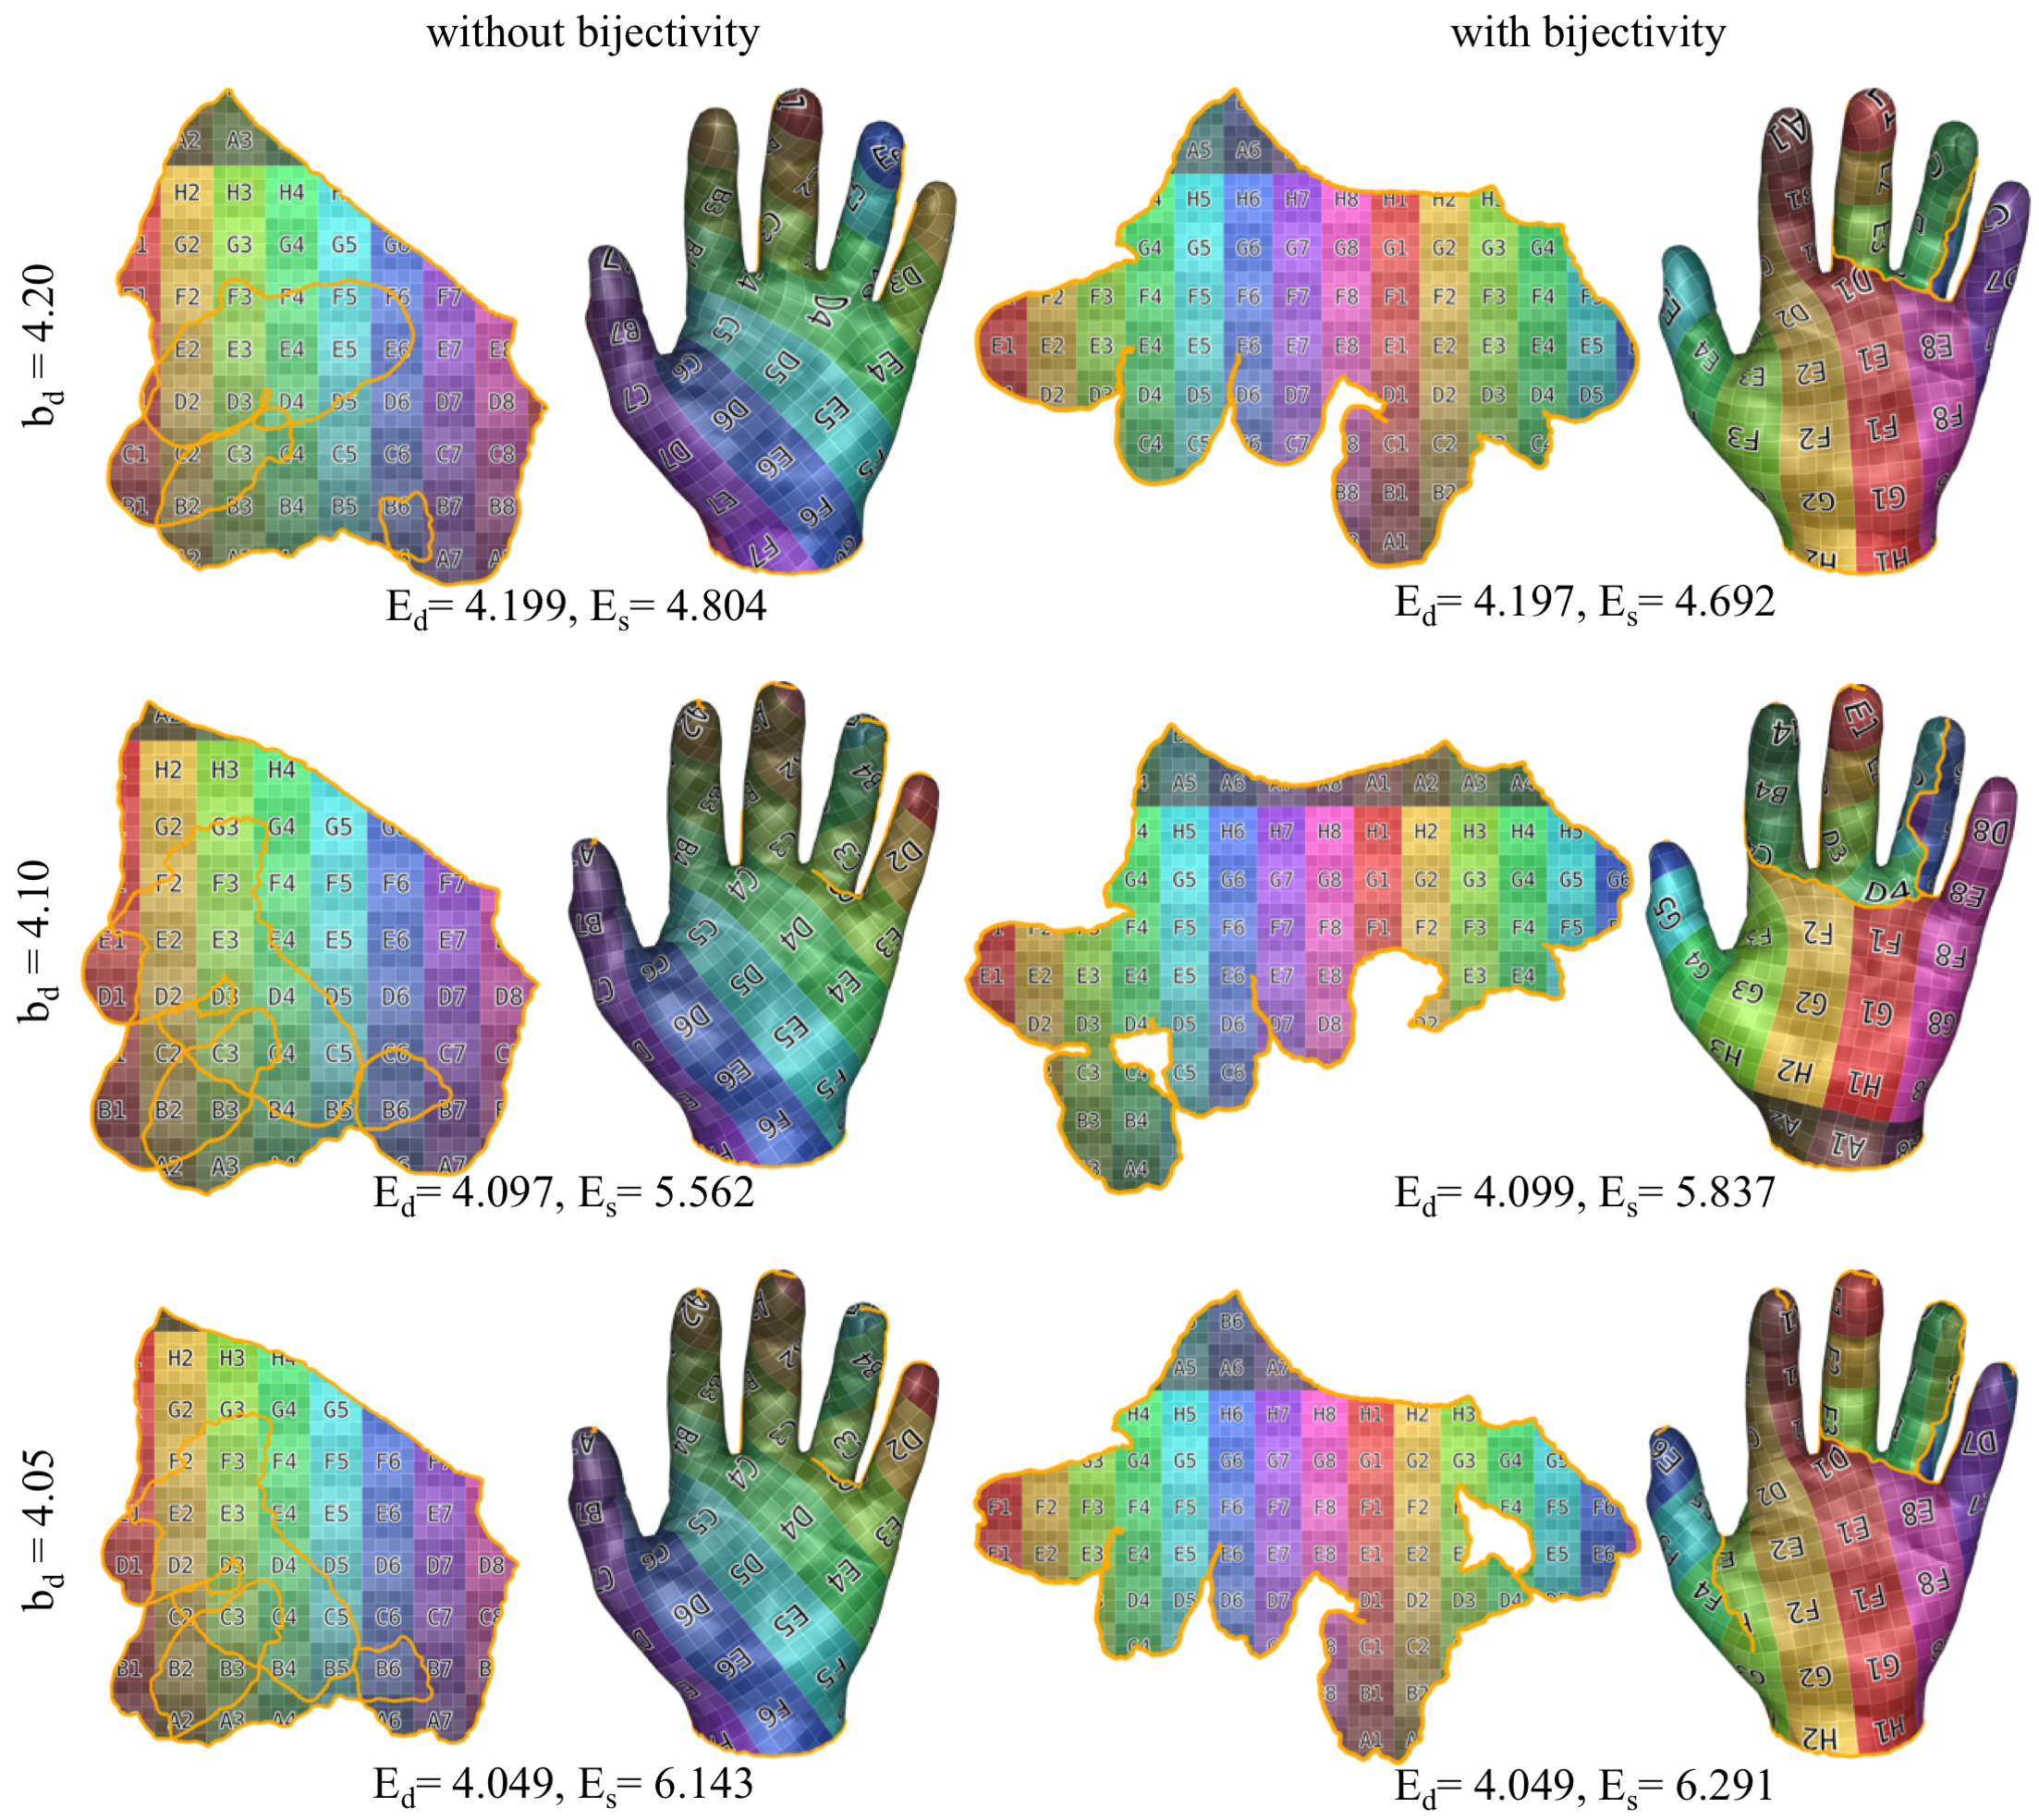
\includegraphics[width=0.48\linewidth]{fig/our_impressive_results_left.png}
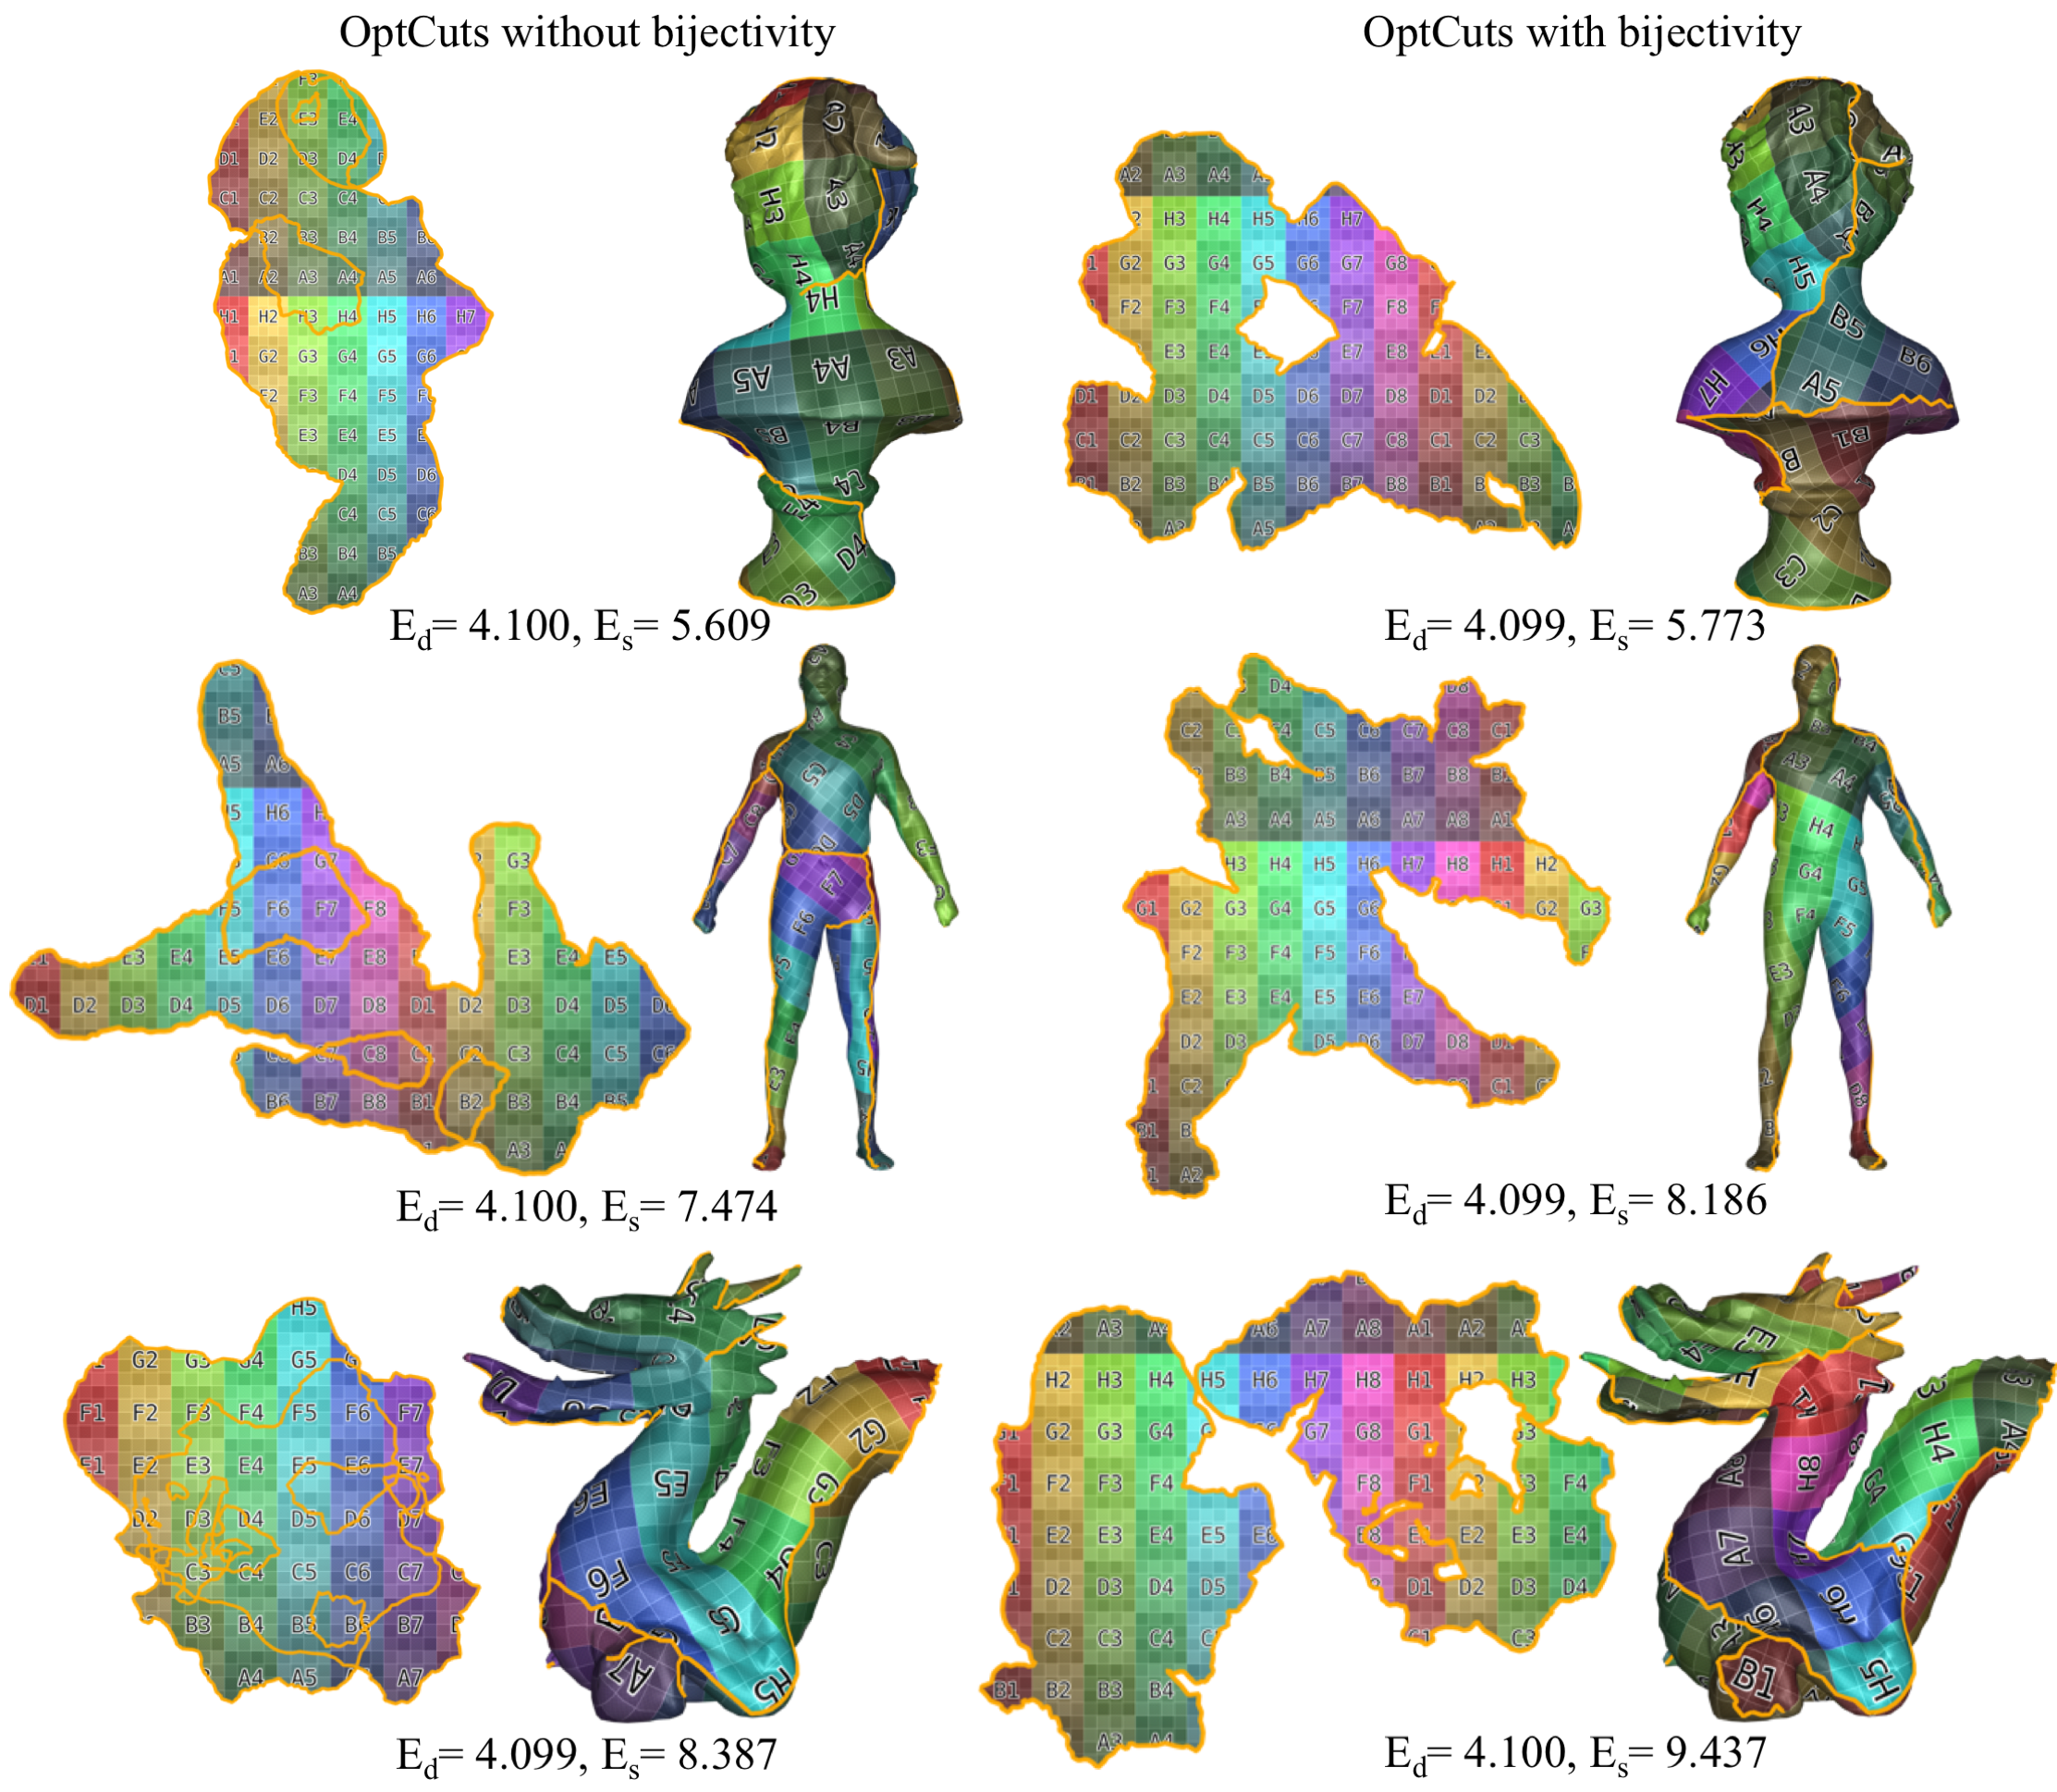
\includegraphics[width=0.5\linewidth]{fig/our_impressive_results_right.png}
\caption{UV maps generated by our methods with/without bijectivity with $b_d$ set to $4.2$, $4.1$, and $4.05$ from top to bottom.}
\label{fig:our_impressive_results}
\end{figure*}
%could also be bunny_i, statue_5, wooden_fish

\paragraph{Evaluation Metric}
We are able to directly use the output normalized $E_{SL}$ as the evaluation metric since our method can generate UV maps with locally optimal seams under a certain distortion bound. This metric can be consistent among comparisons against all methods because given an input surface we are always able to compare the output $E_{SL}$ under the same level of distortion. Moreover, it also fits in well with practical scenarios where the control of distortions are more intuitive to the users and as-short-as-possible seams are expected.

\paragraph{Initial Embedding}
\minchen{[TODO?]}
For closed surfaces, it is important to first obtain an initial seam for our method to construct the initial UV map. To show that we can always find a local optimum with respect to both the UV topology and coordinates regardless of initial embedding, we run our method on an input surface with several randomly picked initial seams and a heuristic initial seam that splits the shortest path between two farthest points on the surface. As demonstrated in Figure~\ref{fig:any_init_ends_well}, we produce high quality UV maps under the given distortion bound for all initializations.

\subsection{Comparison to AutoCuts}

We demonstrate the capabilities of our framework by comparing to the state-of-the-art AutoCuts~\cite{Poranne2017Autocuts}.
AutoCuts obtains high quality UV maps by involving users into the optimization loop. However, when aiming for convenient, fully-automatic methods, the non-smoothness of their Separation energy not only makes it challenging for global parameter settings, but also often end up the optimization with suboptimal results. To show that we automatically generate high quality UV maps without suffering from these issues, we compare our method with a fully automatic version of AutoCuts obtained under the guidance of AutoCuts authors by constructing appropriate homotopy paths with a uniform set of mesh-adaptive parameters. 
Specifically, we used $\lambda = 0.4$ and started with $\delta=100\overline{|e|}^2$ and half it in the beginning of each homotopy iteration until it reaches $10^{-4}\overline{|e|}^2$. Inside each homotopy iteration, we detect convergence by setting a tolerance $\sqrt{3n_t}\times10^{-3}\overline{|e|}$ on the $L^2$ norm of UV coordinate changes. Here $\overline{|e|}$ is the average edge length, $n_t$ is the number of triangles.

Since AutoCuts does not intuitively support generating UV maps with a certain level of distortion, we first run AutoCuts on a batch of input surfaces, and then set their output distortions as $b_d$ in our method for each input. As demonstrated in Table~\ref{tb:comp_AutoCuts}, for both the two versions of our method, we require less time to generate UV maps with same level of distortion but significantly smaller seams. Figure~\ref{fig:ESLBar_compAutoCuts} shows a bar chart comparison on the output $E_{SL}$ of each input surface. Note that we easily enforced bijectivity (Figure~\ref{fig:comp_AutoCuts}), which is only supported in AutoCuts with user assistance on patch manipulation.

\begin{table}[!h]
\centering
\caption{Comparisons between AutoCuts and our methods with/without bijectivity (WB/NB) on 69 input surfaces with $3749$ vertices per input in average. Even with bijectivity, we achieve shorter seam length with less running time.}
\label{tb:comp_AutoCuts}
\begin{tabular}{|c|ccc|ccc|}
\hline
\multirow{2}{*}{method} & \multicolumn{3}{c|}{$E_{SL}$} & \multicolumn{3}{c|}{time (s)} \\ \cline{2-7} 
                        & avg      & min     & max      & avg      & min    & max       \\ \hline
AutoCuts                & 7.5789   & 1.2069  & 24.6816  & 499.9    & 4.0    & 2677.0    \\
ours (WB)               & 5.8114   & 0.8979  & 19.7405  & 304.0    & 6.4    & 1267.7     \\
ours (NB)               & 5.3065   & 0.8992  & 16.1329  & 148.7    & 3.1    & 650.9    \\ \hline
\end{tabular}
\end{table}

\begin{figure}[!h]
\centering
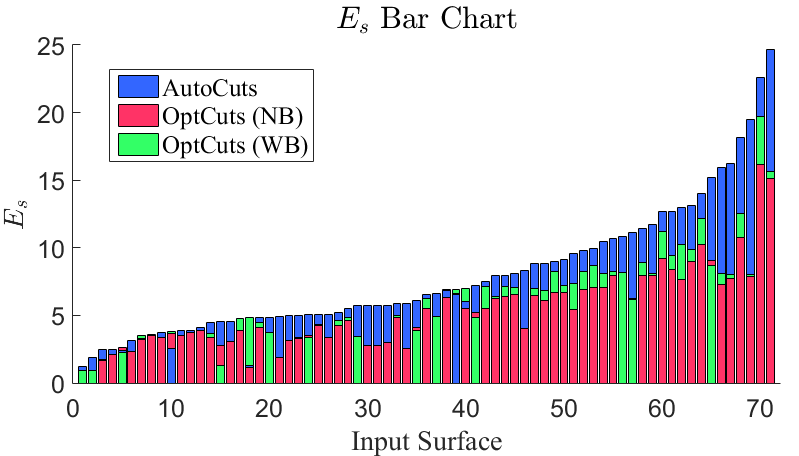
\includegraphics[width=\linewidth]{fig/ESLBar_compAutoCuts.png}
\caption{Normalized seam length $E_{SL}$ bar chart of each example generated by AutoCuts and our method with/without bijectivity. We achieve much shorter seams for almost all the inputs under the same levels of distortion.}
\label{fig:ESLBar_compAutoCuts}
\end{figure}

\begin{figure}[!h]
\centering
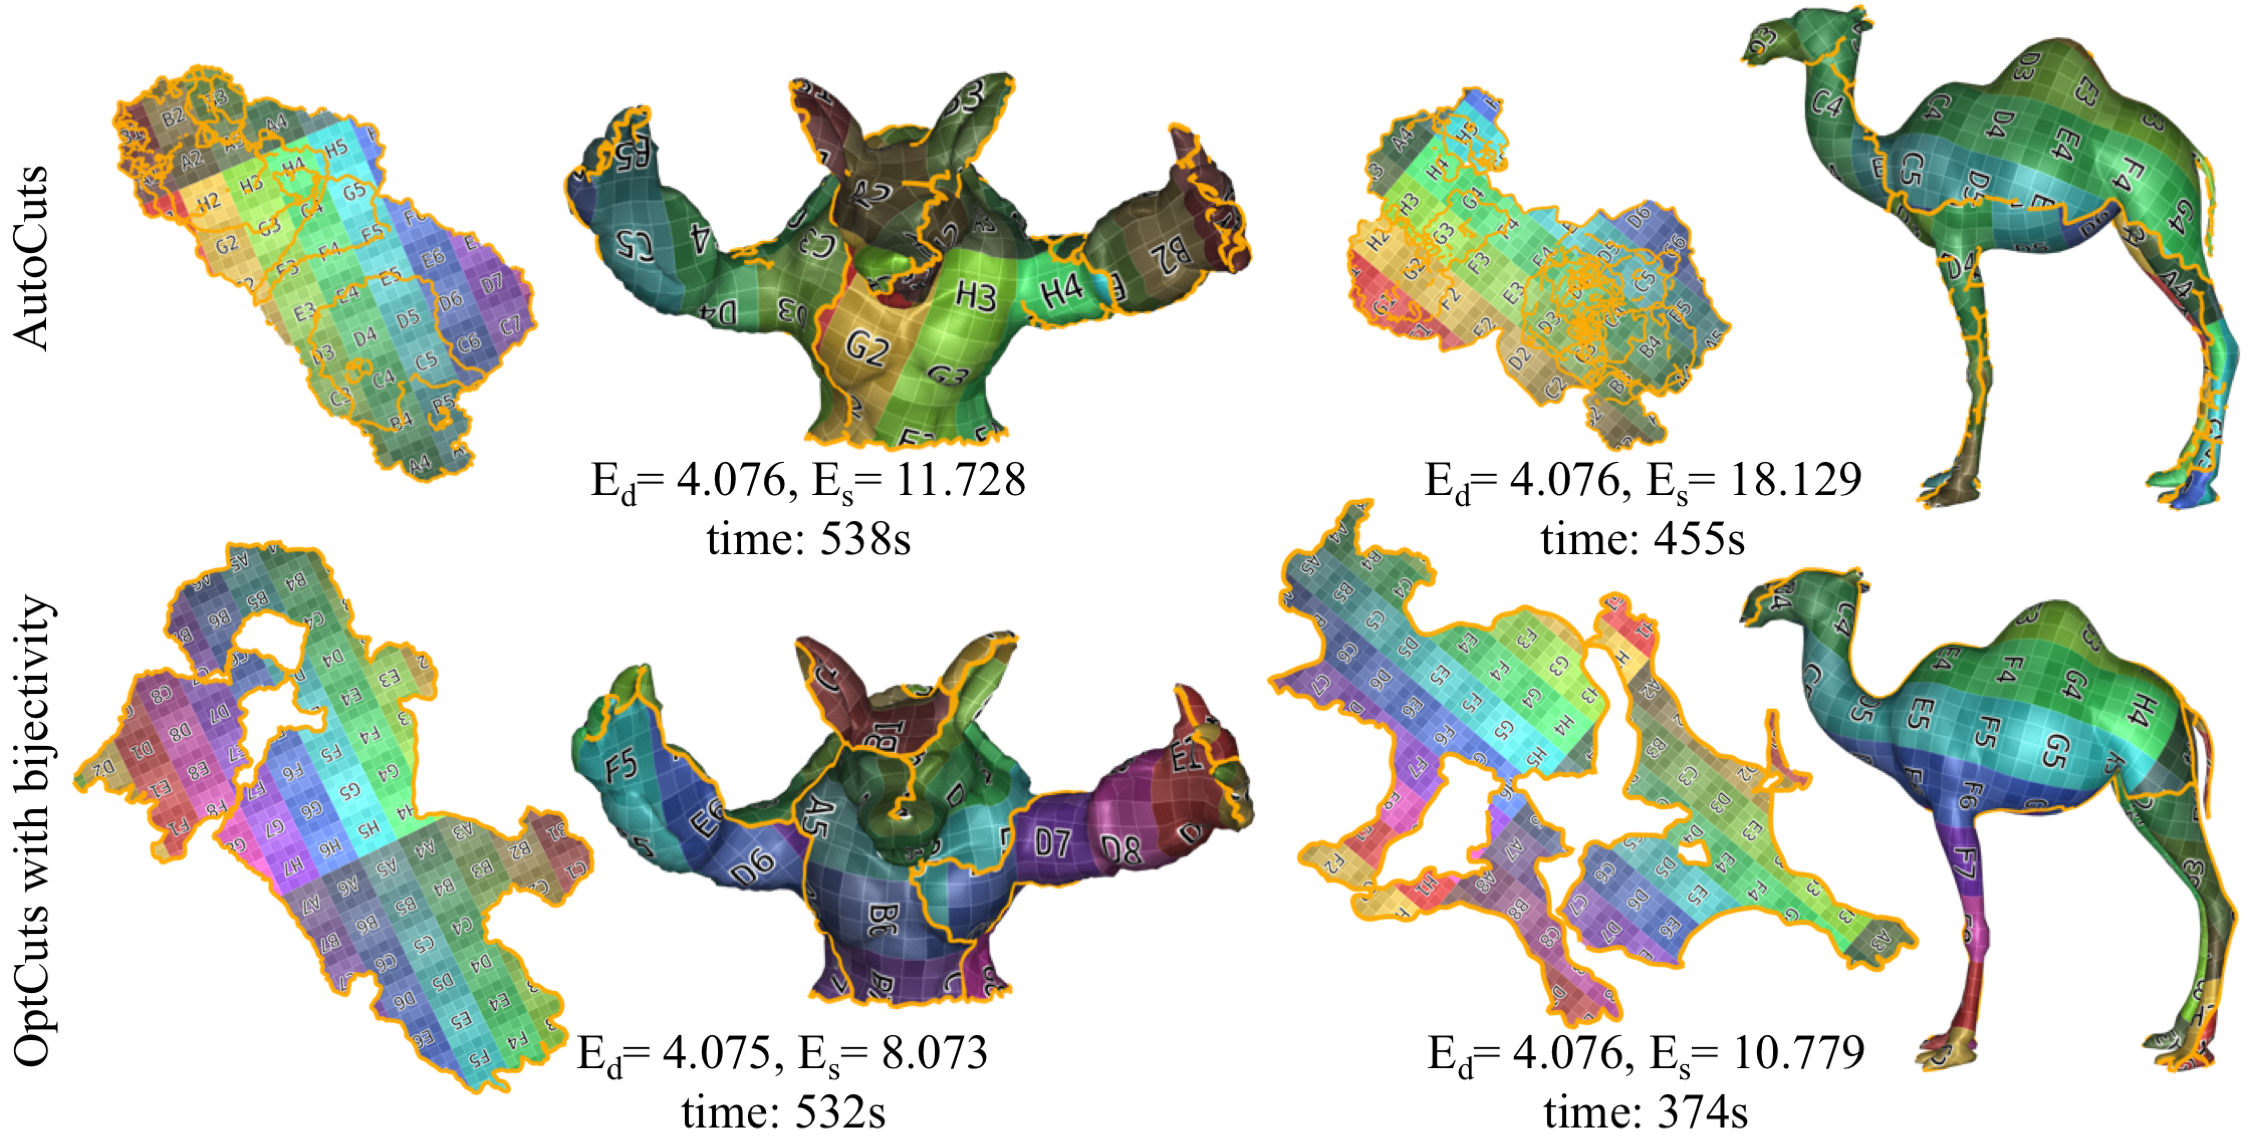
\includegraphics[width=\linewidth]{fig/comp_AutoCuts.png}
\caption{Comparison between AutoCuts (top) and our method (bottom) on the armadillo (left) and camel (right) model, from which we can see that with a single set of parameters, AutoCuts may generate sub-optimal results for some inputs.}
\label{fig:comp_AutoCuts}
\end{figure}
% could also be bone_noInput, bunny_i_f10000, bunny, camel_vova_f10000, cat_noUV, cow_param_closed, dilo, horse, male_2, octopus, wooden_fish, foot_i_f10000, three_man_statue, gargoyle, rgb_dragon, statue_i_1, vase, venus

\paragraph{Scalability}
From the time-resolution scatter plot in Figure~\ref{fig:time_res_compAutoCuts}a, we see that for meshes with higher resolution, our method scales better on running time than AutoCuts.
We further run AutoCuts and our methods on 5 input surfaces obtained by progressively simplifying the original lucy model (48354 vertices) to test scalability. From the trend in Figure~\ref{fig:time_res_compAutoCuts}b, we further see that our method scales better. Besides, the average $E_{SL}$ obtained by our methods with/without bijectivity on the lucy models are $9.236$ and $8.816$ respectively, much smaller than $13.052$ by AutoCuts. Notice that for models with 24200 and 48354 vertices, AutoCuts already run out of memory, since its system size is $6$ times that of ours.

\begin{figure}[!h]
\centering
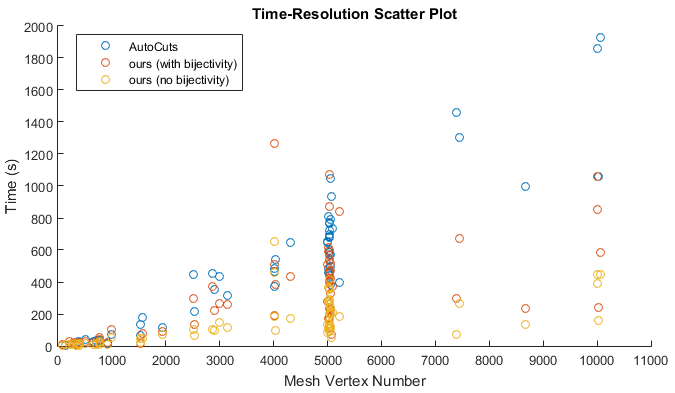
\includegraphics[width=\linewidth]{fig/time_res_compAutoCuts.png}
\caption{Time-resolution scatter plot of a batch of examples (a) and 5 lucy models with different resolutions (b) generated by AutoCuts and our method with/without bijectivity. Note that in (b), there is no data points for AutoCuts on models with 24200 and 48354 vertices due to running out of memory. From the trend, we see that our methods scales better to meshes with higher resolution.}
\label{fig:time_res_compAutoCuts}
\end{figure}


\subsection{Variations}

\paragraph{Regional Seam Placement}
In texture painting applications, users would really like regions with the same semantic meanings stay connected or close to each other on the UV map. If we let users to select those regions on the input surface, we could easily avoid seams in those regions while still achieving bijectivity and similar seam length under the same distortion bound (Figure~\ref{fig:regional_seam_placement}). Without changing our framework, we just need to modify our formulation of $E_s$ by weighting each seam edge using the indicator function $w_{SL}$ provided by the user:
\[ E_s = \hat{E}_{SL} = \sum_{i\in\mathcal{S}} w_{SL,i} E_{SL,i} \quad w_{SL,i} \in [1.0, +\infty] \]

\begin{figure}[!h]
\centering
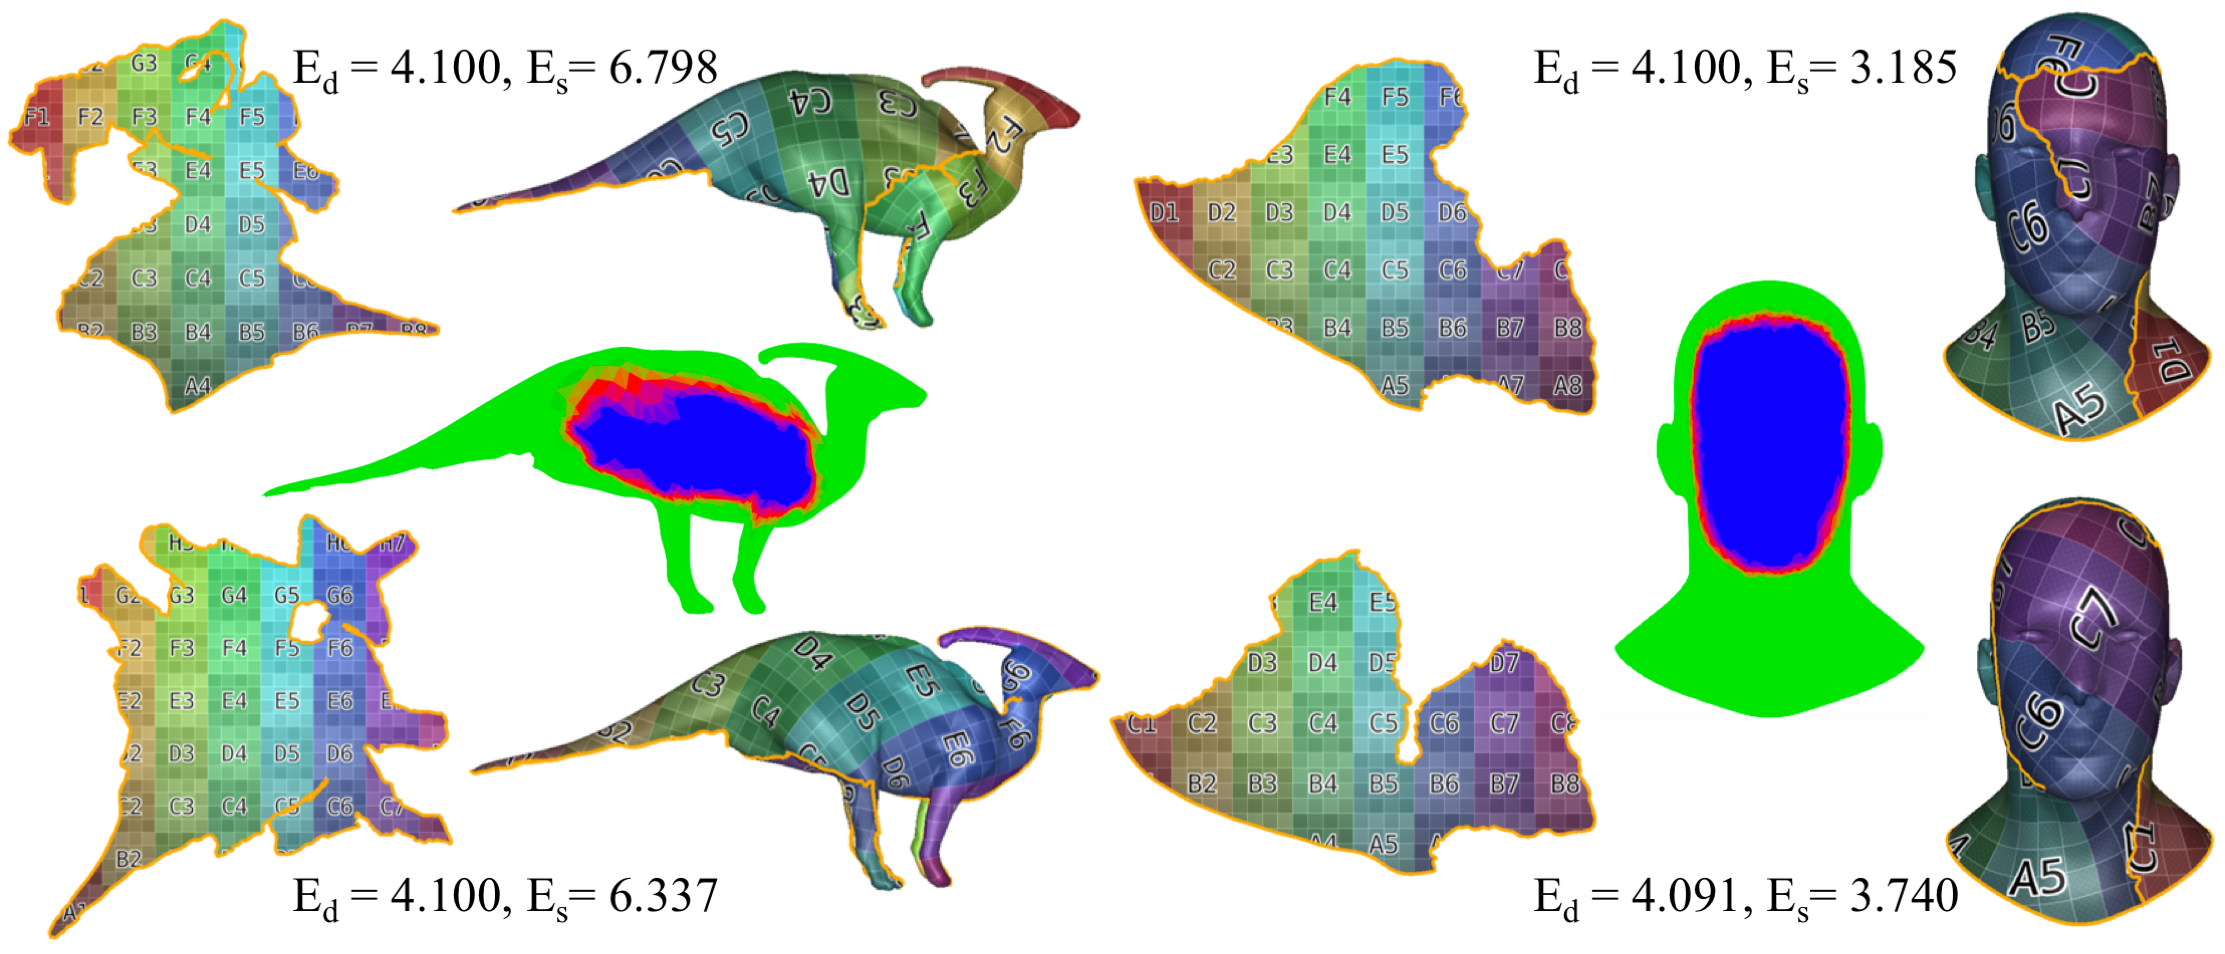
\includegraphics[width=\linewidth]{fig/regional_user.png}
\caption{Two examples of user controlled regional seam placement. Up to bottom: UV maps generated by the standard version of our method with bijectivity and $b_d = 4.1$, user preference on regional seam placement (blue means seams are less wanted), UV maps generated by the variation of our method supporting the given user preference (with bijectivity and $b_d = 4.1$). For the left dilo model, we achieve shorter seam length with the regional constraints. This can also happen when involving our bijectivity constraints, since our method is searching for local optimum.}
\label{fig:regional_seam_placement}
\end{figure}

% \paragraph{Conformal Parameterization}
% Using a conformal energy~\cite{Hormann2000MIPS,Sheffer2005ABFPP} for $E_d$ will achieve joint seam placement and conformal parameterization. Figure~\ref{fig:conformal_vs_isometry} shows some results with $E_d = E_{ABForMIPS}$~\cite{} compared to results with $E_d = E_{SD}$, where different seams are generated while our framework stays the same.

\paragraph{Different Cutting Strategy}
The cutting strategy in the topology descent steps essentially build up the structure of the UV topology graph $\mathcal{G}_T$. By considering local topological operations, we built a dense graph connecting almost all the possible UV topologies and then reduce the search complexity by filtering. Alternatively, one can consider building $\mathcal{G}_T$ using only a sparse set of UV topologies and more aggressive topological operations, like the extremity-boundary (EB) cut applied in Geometry Images~\cite{Gu2002Geometry}.

We could alternatively apply EB strategy in our framework without bijectivity constraints by simply alternating the cut with distortion minimization processes, and stop right after $b_d$ is reached. This variation of our method reaches identical distortion bounds with very similar seam length compared to our standard method, but is much faster since the EB cut can be decided nearly instantly (Table~\ref{tb:comp_GI}). However, when we set smaller distortion bounds, the quality of the seams by EB cut drops since extremities are not that obvious on a nearly isometric UV map (Figure~\ref{fig:comp_GI}).

\begin{table}[!h]
\centering
\caption{Comparison between the standard version of our method and using EB cutting strategy in our framework, both without bijectivity constraints. We run the two methods on 70 input surfaces with $3721$ vertices per input in average. With EB cutting strategy, we achieve similar seam length but much faster.} 
\label{tb:comp_GI}
\begin{tabular}{|c|c|ccc|ccc|}
\hline
\multirow{2}{*}{$b_d$} & \multirow{2}{*}{method} & \multicolumn{3}{c|}{$E_{se}$} & \multicolumn{3}{c|}{time (s)} \\ \cline{3-8} 
                       &                         & avg      & min     & max      & avg       & min    & max      \\ \hline
\multirow{2}{*}{4.2}   & ours                    & 3.819   & 0.080  & 14.545  & 87.0   & 0.3 & 417.8 \\
                       & ours(EB)                & 3.868   & 0.159  & 14.929  & 13.0   & 0.1 & 72.1  \\ \hline
\multirow{2}{*}{4.1}   & ours                    & 4.709   & 0.752  & 17.980  & 137.5  & 0.9 & 886.9 \\
                       & ours(EB)                & 4.795   & 1.207  & 16.895  & 17.0   & 0.1 & 87.2  \\ \hline
\multirow{2}{*}{4.05}  & ours                    & 6.142   & 0.277  & 21.566  & 213.2  & 3.9 & 1398.1   \\
                       & ours(EB)                & 6.335   & 0.328  & 23.051  & 24.1   & 0.1 & 115.4 \\ \hline
\end{tabular}
\end{table}

\begin{figure}[!h]
\centering
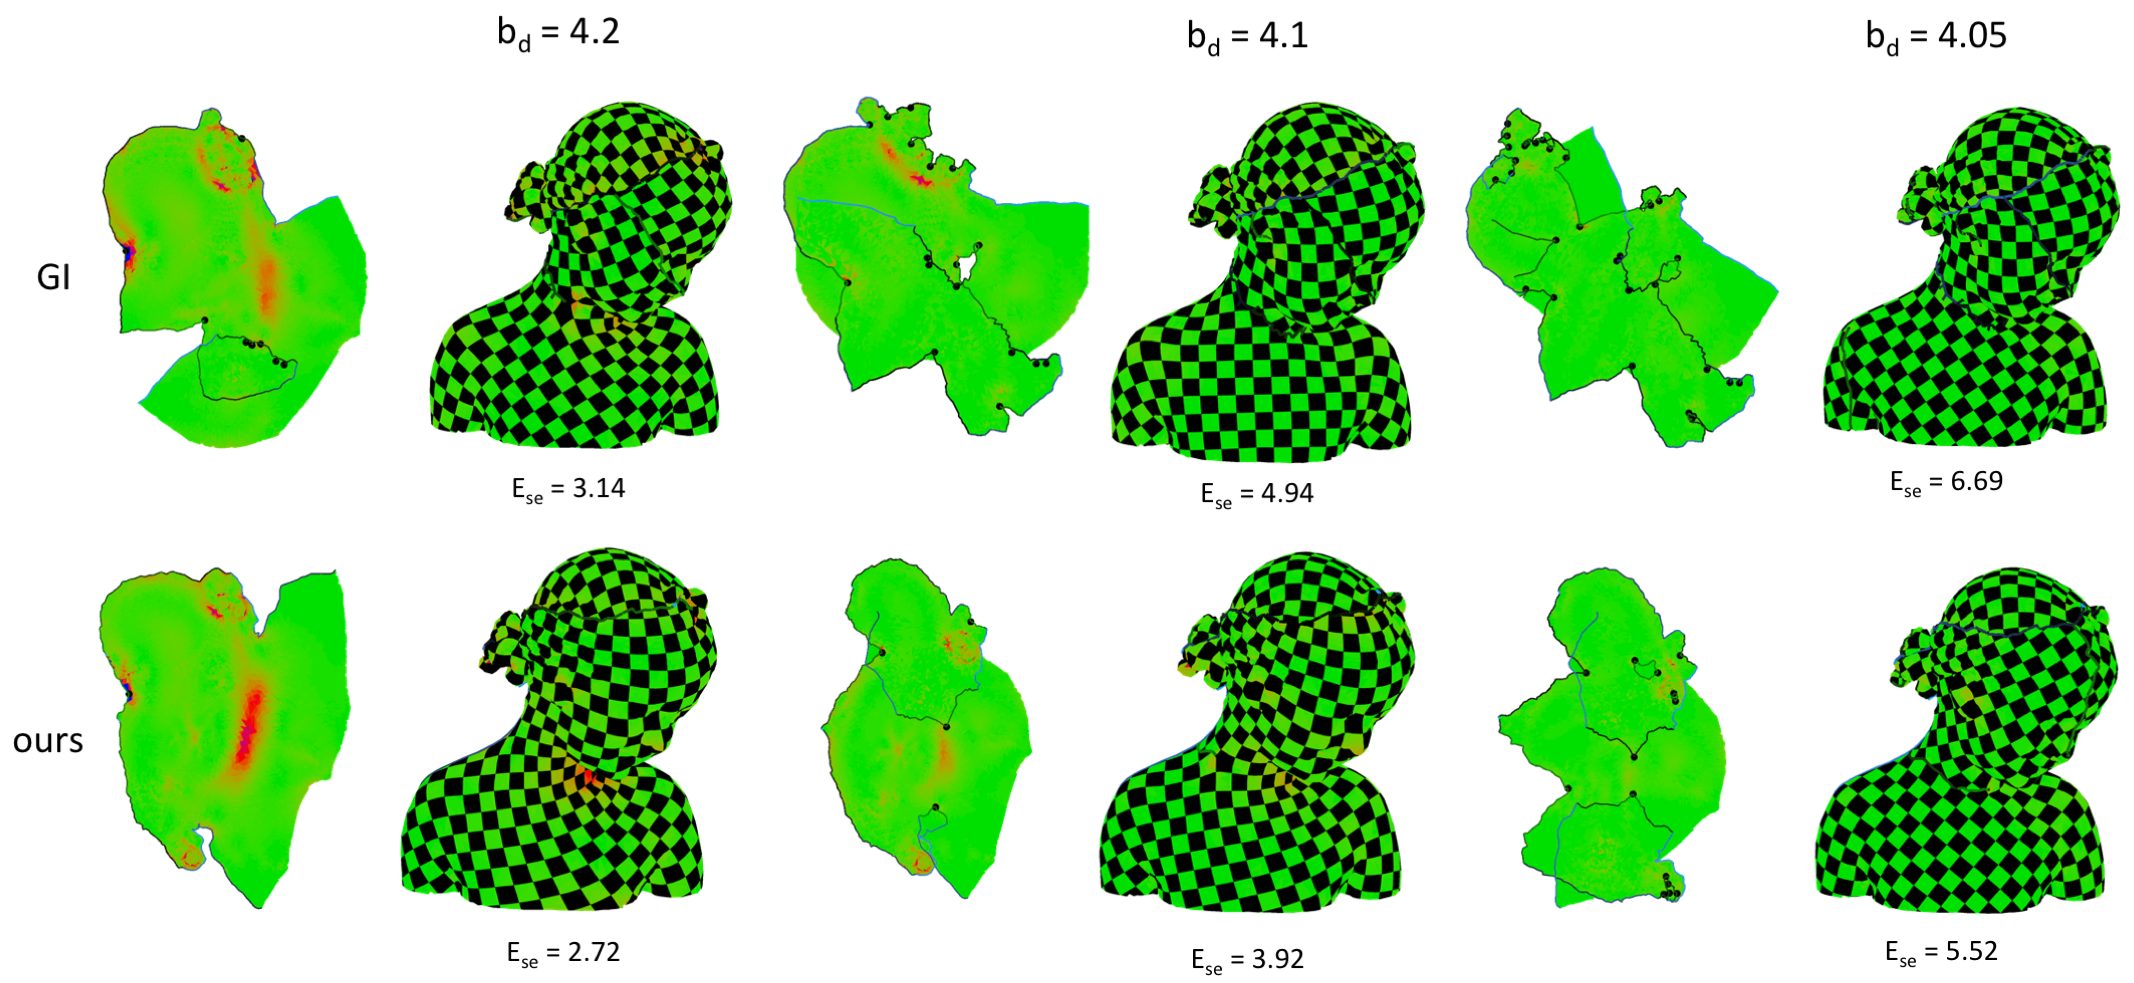
\includegraphics[width=0.8\linewidth]{fig/comp_GI.png}
\caption{Comparison between the standard version of our method (left) and using EB cutting strategy in our framework (right), both without bijectivity constraints. EB cutting stategy is very efficient in early stages (a, b), but it does not work well when the UV map gets closer to isometric where extremities are not standing out (c).}
\label{fig:comp_GI}
\end{figure}
% also could be face_f10000, male_body_i_f10000, statue_4_i_f10000, statue_5_i_f10000, bimba_i_f10000

\paragraph{Warm Start}
Although we obtain high quality results given any initial embedding, the starting point does affect which local optimal point we will reach. Hence, it is meaningful to explore our method starting from initial seams with global observations. This will also benefit practical scenarios for improving preliminary UV maps while stay close to it.

If we take the output seams by our method with EB strategy to construct the initial embedding, we can improve the seam quality towards the nearby local optimal point while still satisfying the same distortion bound. Even if we add bijectivity constraints back, we still achieve shorter seam length compared to both our standard method without bijectivity and our method with EB strategy. (Figure~\ref{fig:comp_GI_outputAsInit}).

\begin{figure}[!h]
\centering
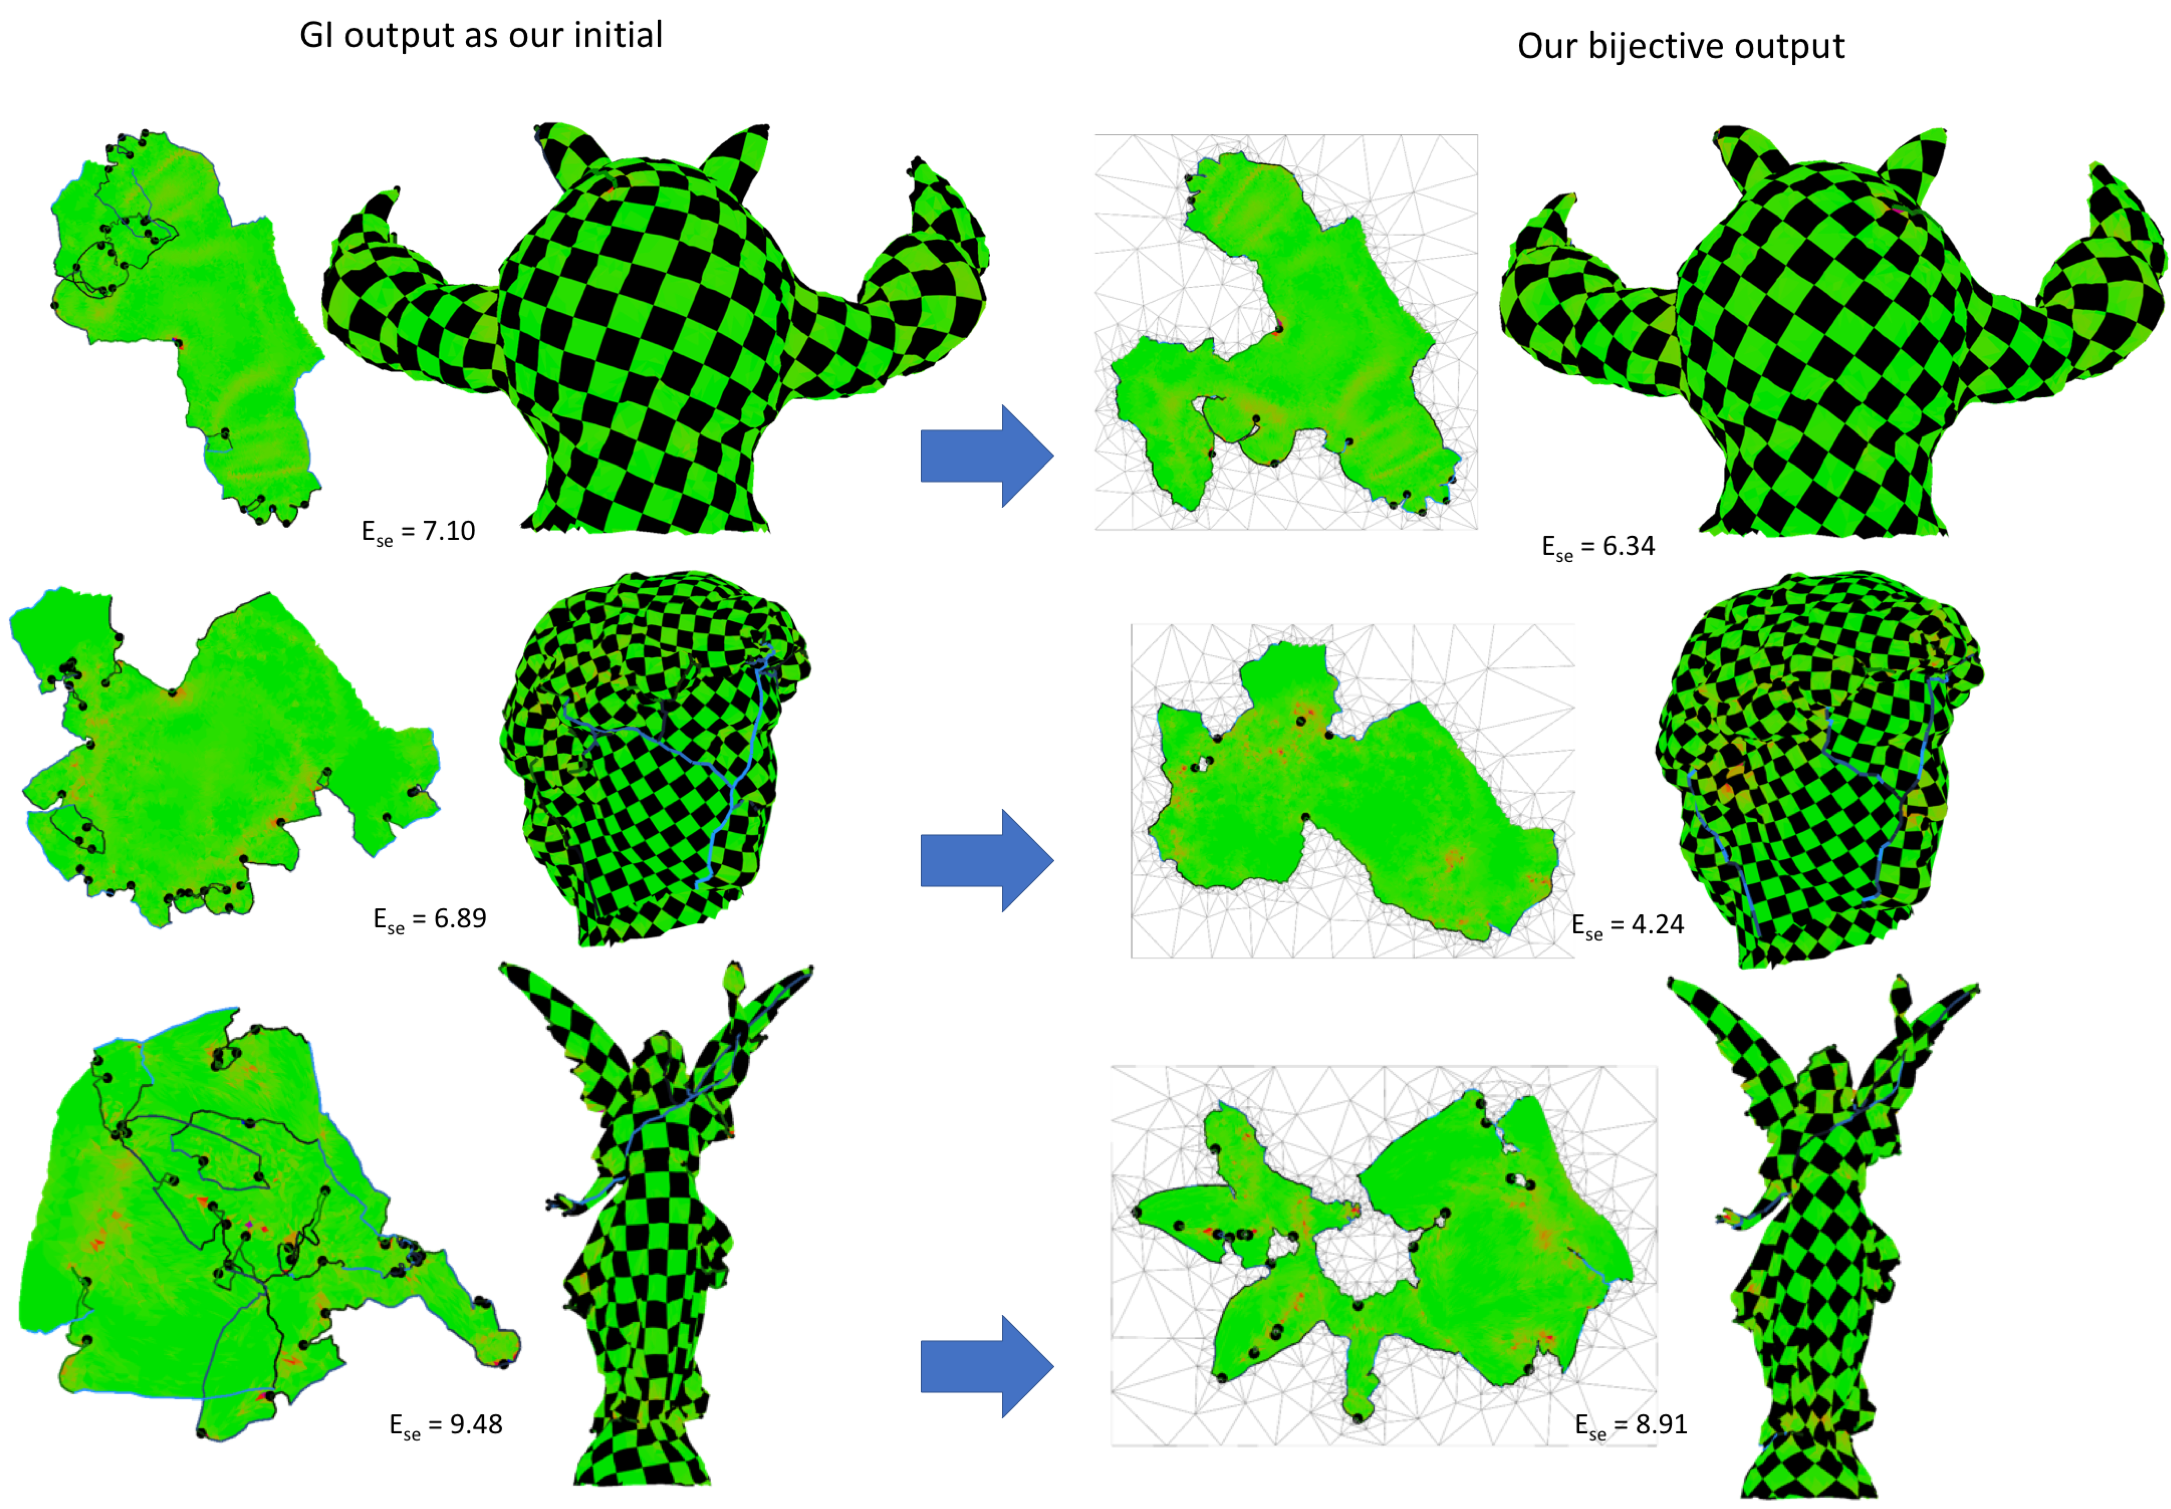
\includegraphics[width=\linewidth]{fig/comp_GI_outputAsInit.png}
\caption{Using output seams by our method with extremity-boundary cutting strategy at $b_d = 4.1$ (a) as our initial UV map, we improve seam quality, reaching a locally optimal seam configuration under the given distortion bound even with bijectivity constraints (b). This seam length is also shorter than results obtained by our standard method without bijectivity (c).}
\label{fig:comp_GI_outputAsInit}
\end{figure}
% also could be bimba, bunny

Seamster~\cite{Sheffer2002Seamster} is another classic seam cutting method worth considering for warm start. With Seamster's best output seams on the cow and triceraptop model, we obtain UV maps by minimizing $E_{SD}$ with bijectivity constraints (Figure~\ref{fig:comp_Seamster}a), and use them for warm start, setting their distortions as the upper bounds. As demonstrated in Figure~\ref{fig:comp_Seamster}b, we achieve shorter seam length while maintaining the distortion bound and bijectivity. This seam length is also shorter than running our standard method without bijectivity from standard initialization (Figure~\ref{fig:comp_Seamster}c).

\begin{figure}[!h]
\centering
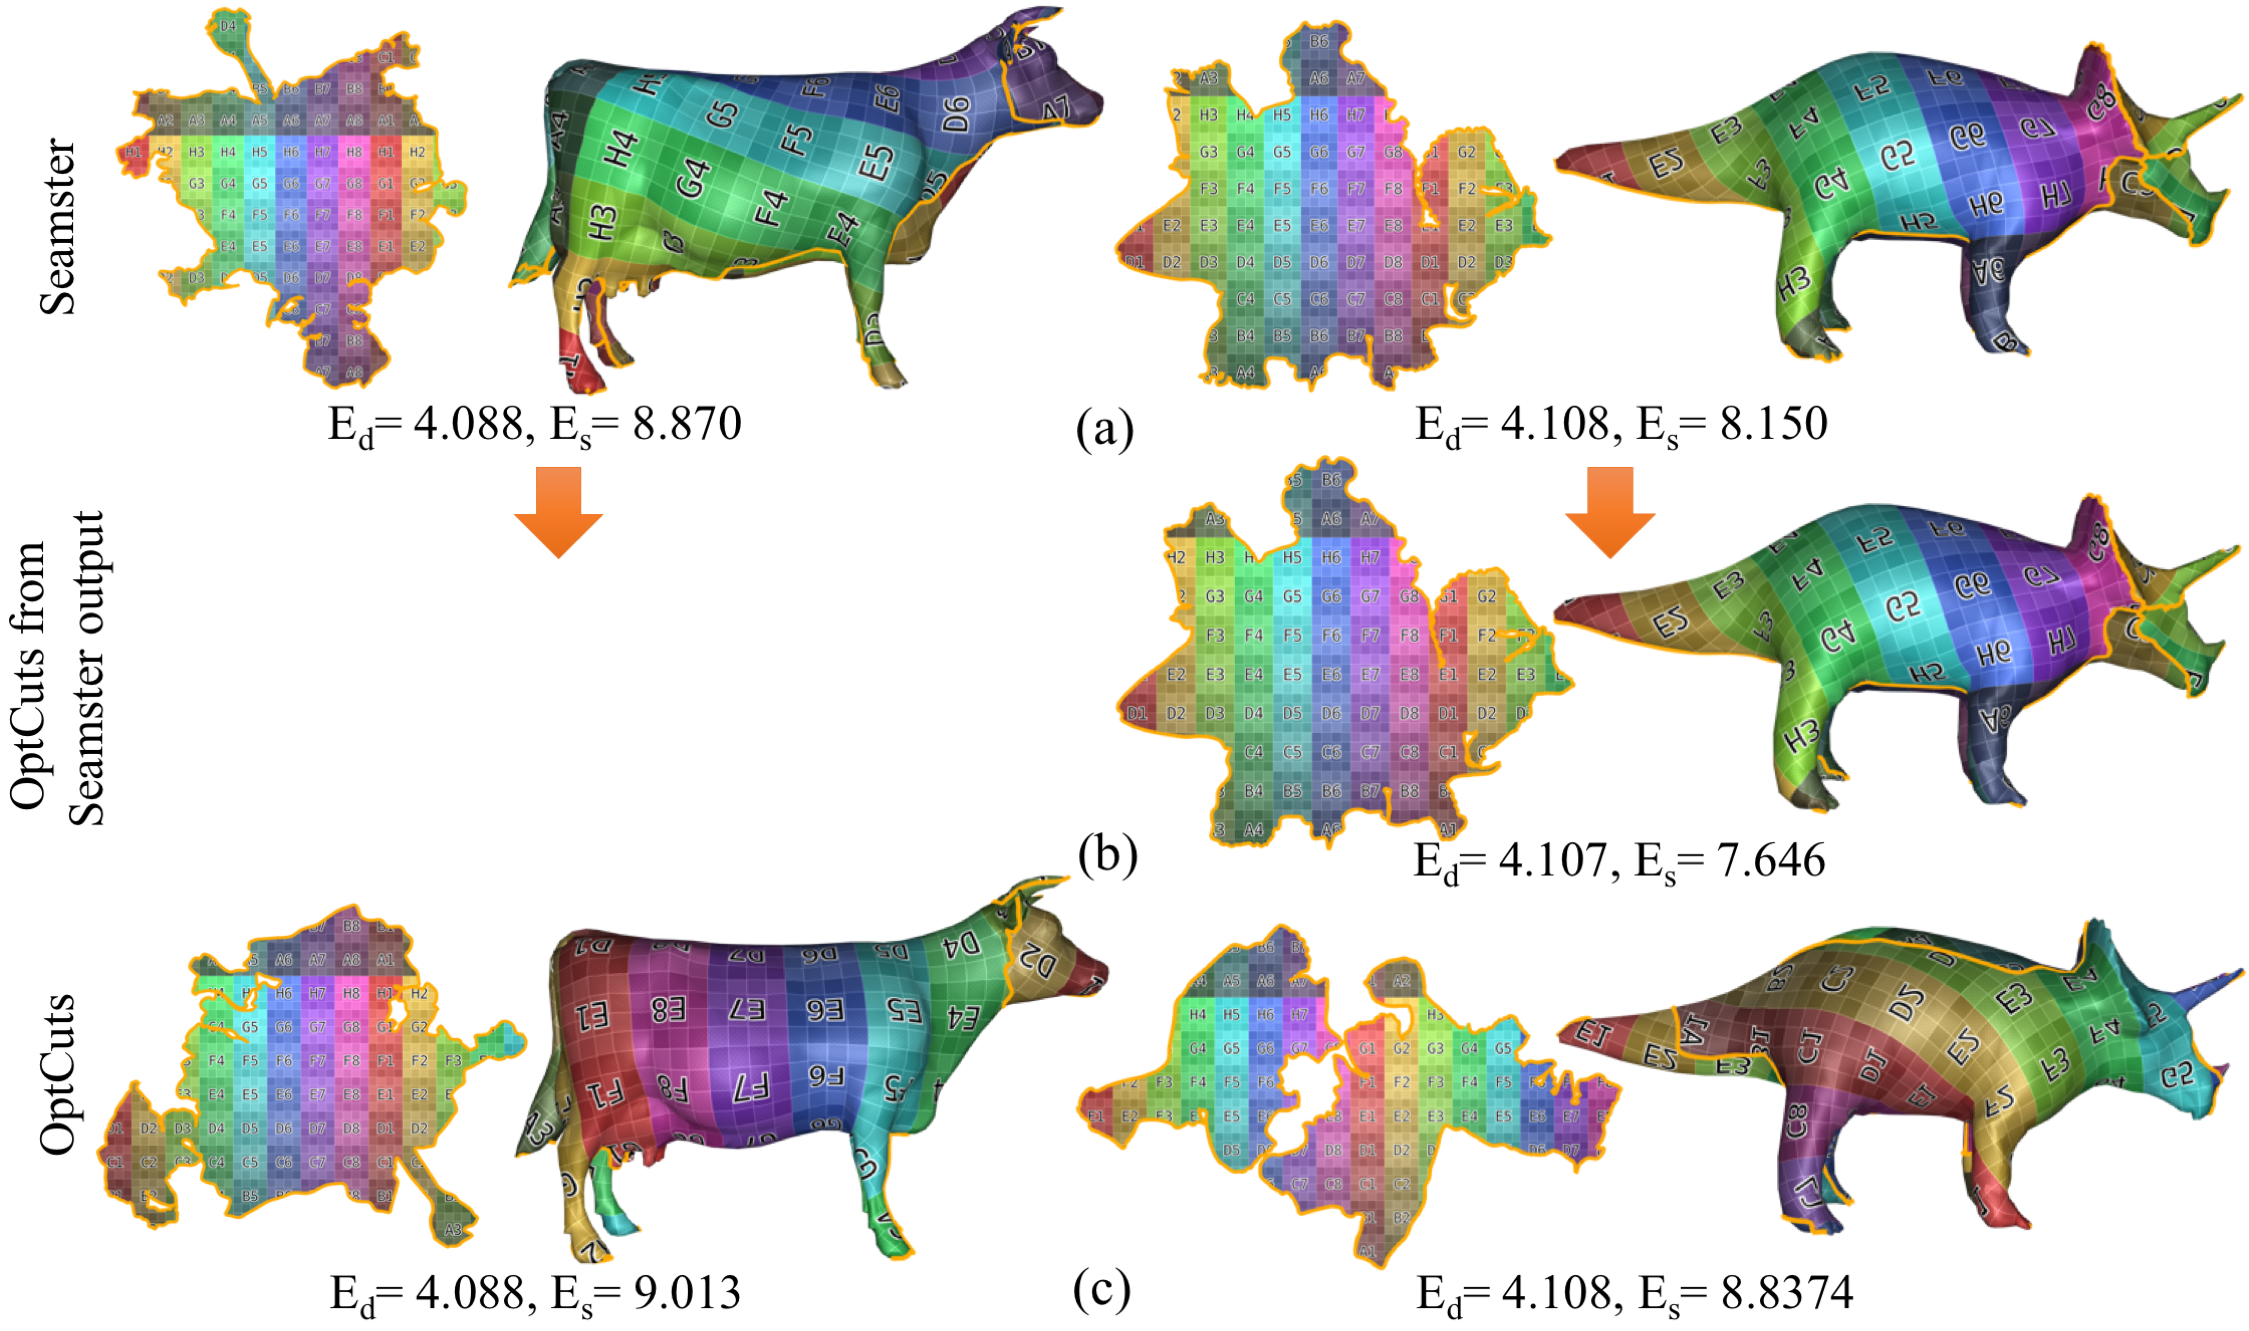
\includegraphics[width=\linewidth]{fig/comp_Seamster.png}
\caption{\minchen{[trouble stitching cow mesh together while maintaining the UV coordinates, will fix soon]} Starting from UV maps obtained by using Seamster's best output seams (a), we improve seam quality, reaching a locally optimal seam configuration while maintaining the distortion and bijectivity (b). This seam length is also shorter than running our standard method without bijectivity from standard initialization (c).}
\label{fig:comp_Seamster}
\end{figure}

For Seamster, user need to set the size of local regions for measuring extremity, which is a mesh and shape dependent parameter that requires fine tuning. Even our method with standard initialization achieves similar seam length without any user assistance.
